\documentclass{report}
\usepackage[T1]{fontenc}
\usepackage[utf8]{inputenc}
\usepackage[francais]{babel}
\usepackage{amsmath}
\usepackage{graphicx}
\graphicspath{{Figures/}}
\usepackage[backend=biber,style=authoryear,bibencoding=utf8]{biblatex}
\addbibresource{biblio.bib}
\usepackage[colorlinks,linkcolor=blue]{hyperref}




\begin{document}
\chapter{L'actine}

L'actine est une protéine ubiquitaire conservée chez tous les eucaryotes, exprimée dans tous les types cellulaires. 
Ses fonctions sont multiples et variées et se divisent en deux catégories principales, les fonctions mécaniques et les fonctions régulatrices. 

Elle se présente dans la cellule sous deux formes principales : en monomères (Actine G pour globulaire) ou en filaments (Actine F). 
Elle interagit avec un grand nombre de protéines appelées Actin-Binding Proteins. 

L'actine est un composant du cytosquelette prenant la forme d'un réseau de filaments très dynamique. La rigidité d'une cellule et sa motilité sont majoritairement contrôlées par l'organisation du cytosquelette d'actine. 

Mais l'actine est également un composant des trois ARN Polymérases PolI, PolII et PolIII, qui transcrivent l'ADN en ARN pendant la première étape de l'expression du génome ( \cite{Ye} \cite{Hoffman} \cite{Hu}). 
Elle est indispensable à la réorganisation de la chromatine qui précède l'expression (revue par \cite{Farrants}) mais aussi à l'export de l'ARN (\cite{hofmann_2001}).  

L'association de ces rôles mécaniques et biologiques fait de l'actine un acteur de choix dans l'interface entre les signaux mécaniques et les signaux biologiques. 

Dans le corps, l'actine a des fonctions spécifiques dans un grand nombre d'organes, comme la contraction des muscles, l'organisation des dendrites et des axones des neurones, le fonctionnement des plaquettes ou de l'appareil auditif. 



\section{Actine G}

\begin{figure}
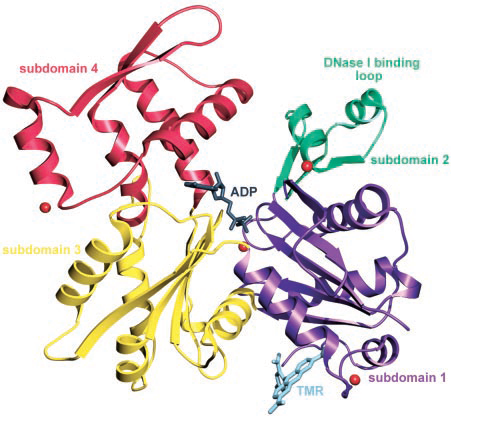
\includegraphics[scale=0.7]{Actine_dominguez.png}
\caption{Cristallisation d'un monomère d'actine ADP, d'après \cite{otterbein_crystal_2001}}
\end{figure}

Chez les mammifères, l'actine est codée par 6 gènes qui peuvent donner une trentaine de molécules différentes par le jeu de l'épissage. 
Elles sont divisées en trois familles : les actines $\alpha$ qui sont exprimées dans les muscles cardiaques, lisses et squelettiques, les actines $\beta$ et $\gamma$ exprimées dans les autres types cellulaires.
Les différentes formes d'actine sont très proches en séquence, mais ne peuvent pas complètement se substituer les unes aux autres. Toutes les formes peuvent s'incorporer dans les filaments. 

La protéine transcrite a un poids moléculaire de 42 kDa, et est produite en grande quantité dans les cellules, où elle pèse environ pour 1 à 5 \% de la masse protéique, mais cela peut aller jusqu'à 15\% de la masse d'une cellule musculaire. 

\subsection{Structure}
La structure moléculaire de l'actine a été observée un grand nombre de fois, en cristallisation avec différents ABP comme la Dnase, la latrunculine ou la profiline. 


Elle est composée de 4 sous-domaines organisés en deux lobes. Les sous-domaines 2 et 4 forment l'extrémité - du filament, les sous-domaines 1 et 3 forment l'extrémité +. Entre les deux lobes se trouve le site de liaison à l'ATP. 
À côté de ce site se trouve une zone d'interaction avec les cations divalents (Ca$^{2+}$ ou Mg$^{2+}$). 

Dans le sous-domaine 2 se trouve une structure de 8 acides aminés appelée Dnase binding loop, désorganisée dans la plupart des cristallisations de l'actine mais organisée en feuillet $\beta$ lorsqu'elle est liée à la Dnase. Au centre de cet élément se trouve une méthionine en position 44 qui peut être oxydée par la protéine MICAL, dont je reparlerai plus en détail plus loin dans ce chapitre et dans le chapitre suivant. 

\subsection{L'actine est une ATPase}

L'actine, après sa fabrication, n'est prête à jouer son rôle qu'avec l'ajout d'une ATP au centre de sa structure.
En plus de ses deux formes, globulaire ou filamenteuse, l'actine est capable d'hydrolyser l'ATP en ADP.

Les deux formes d'actine, ATP et ADP sont capables de former des filaments et de s'incorporer à des filaments. 


\subsection{Localisation et transport}

L'actine a longtemps été étudiée pour son rôle dans le cytoplasme, en tant que composant du cytosquelette. Cependant de l'actine est également présente dans le noyau de la cellule, où elle a des rôles essentiels. 
L'actine peut polymériser dans les deux compartiments (\cite{mcdonald_nucleoplasmic_2006},\cite{baarlink_nuclear_2013}), bien que l'on ne trouve pas de grands filaments organisés dans le noyau. 

L'actine est à une taille intermédiaire pour les pores nucléaires : elle n'est pas tout à fait assez petite pour diffuser facilement à travers. Elle est donc transportée activement entre le noyau et le cytoplasme. 
Son import nécessite la liaison à la cofiline, et est médiée par l'importine 9 (\cite{dopie_active_2012}). Son export nécessite la profiline et est médiée par l'exportine 6 (\cite{dopie_active_2012}).



\subsection{Oxydation de l'actine}

Les protéines MICAL sont capables d'ajouter deux atomes d'oxygène sur la Méthionine qui se trouve en 44e position de la la chaîne d'acides aminés de l'actine. Cet acide aminé est au centre d'une zone de la protéine qui relie les monomères dans un filament. 
L'oxydation spécifique de cet acide aminé déstabilise les filaments et l'actine oxydée est incapable de se lier à d'autres actines pour former de nouveaux filaments \cite{hung_direct_2011}. 



\subsection{Protéines interagissant avec l'actine G}

 La profiline est une petite protéine (autour de 15kDa) qui peut se lier à l'actine G par son extrémité +, l'empêchant de former un nouveau filament ou de se lier à l'extrémité - d'un filament existant. 
Bien qu'elle se lie au monomère, son action est globalement favorable à la croissance des filaments \cite{pollard_1984}. 
La profiline facilite le remplacement d'une ADP par une ATP dans le monomère auquel elle est attachée. 
Or l'actine ATP polymérise mieux que l'actine ADP, l'action de la profiline va donc recycler l'actine ADP dépolymérisée des anciens filaments en actine ATP prête à allonger de nouveaux filaments. 
De plus, les élongateurs de filaments comme les formines et VASP vont préférentiellement utiliser de l'actine liée à la profiline pour faire croître les filaments \cite{Ferron},\cite{romero}. 
La profiline joue également un rôle dans la localisation de l'actine : l'exportine 6 va se lier spécifiquement au complexe actine-profiline et le faire passer de l'intérieur vers l'extérieur du noyau (\cite{dopie_active_2012}).


Les thymosines $\beta 4$ sont de toutes petites protéines d'environ 5kDa dont le rôle principal est de maintenir un réservoir d'actine monomérique \cite{Safer}. Elles se lient principalement aux actines ATP et les empêchent de polymériser. 

Les CAP (Adenylate Cyclase Associated Protein) sont également des catalyseurs de l'échange d'un ADP contre un ATP dans les monomères d'actine\cite{makkonen}. 

Les cofilines sont une famille de petites protéines qui lient à l'actine G et à l'actine F. Elles ont une préférence pour l'actine ADP. 
Le complexe cofiline-actine est plus facilement recruté par les CAP, qui vont  dissocier le complexe et remplacer l'ADP par une ATP sur l'actine. 
Les cofilines sont suffisamment petites pour passer par les pores nucléaires par diffusion, elles sont cependant dotées d'un signal de localisation nucléaire. Cela leur permet d'être importées dans le noyau lorsqu'elles sont liées à d'autres protéines plus massives. 
Ainsi, le complexe cofiline-actine est importé dans le noyau par l'importine 9 (\cite{dopie}).

L'actine bloque l'activité de la DNase I, une enzyme qui coupe l'ADN en fragments de 4 paires de bases de manière non spécifique. La DNase I se lie à l'actine globulaire avec une grande affinité, alors qu'elle ne se lie que très peu à l'actine F, c'est pourquoi elle est souvent utilisée pour la détection de l'actine G en immunofluorescence. 

Les Myocardin-Related Transcription Factors sont des cofacteurs de transcriptions qui peuvent former un complexes avec trois ou cinq monomères d'actine \cite{mouilleron_molecular_2008}. Leur rôle n'est pas de réguler l'équilibre dynamique de l'actine mais d'agir comme un détecteur de la concentration de monomères d'actine disponibles. 
En fonction de l'état de polymérisation du cytosquelette, les MRTF vont réguler l'activité d'un facteur de transcription contrôlant les gènes de l'actine et d'un grand nombre d'ABP qui régulent sa dynamique. 
Les MRTF sont un maillon d'une boucle de rétro-action qui contrôle la dynamique de l'actine à long terme par l'expression des gènes \cite{salvany_core_2014}. 
Les mécanismes détaillés de ce contrôle et ses conséquences seront décrits dans le chapitre 3. 

\begin{figure}
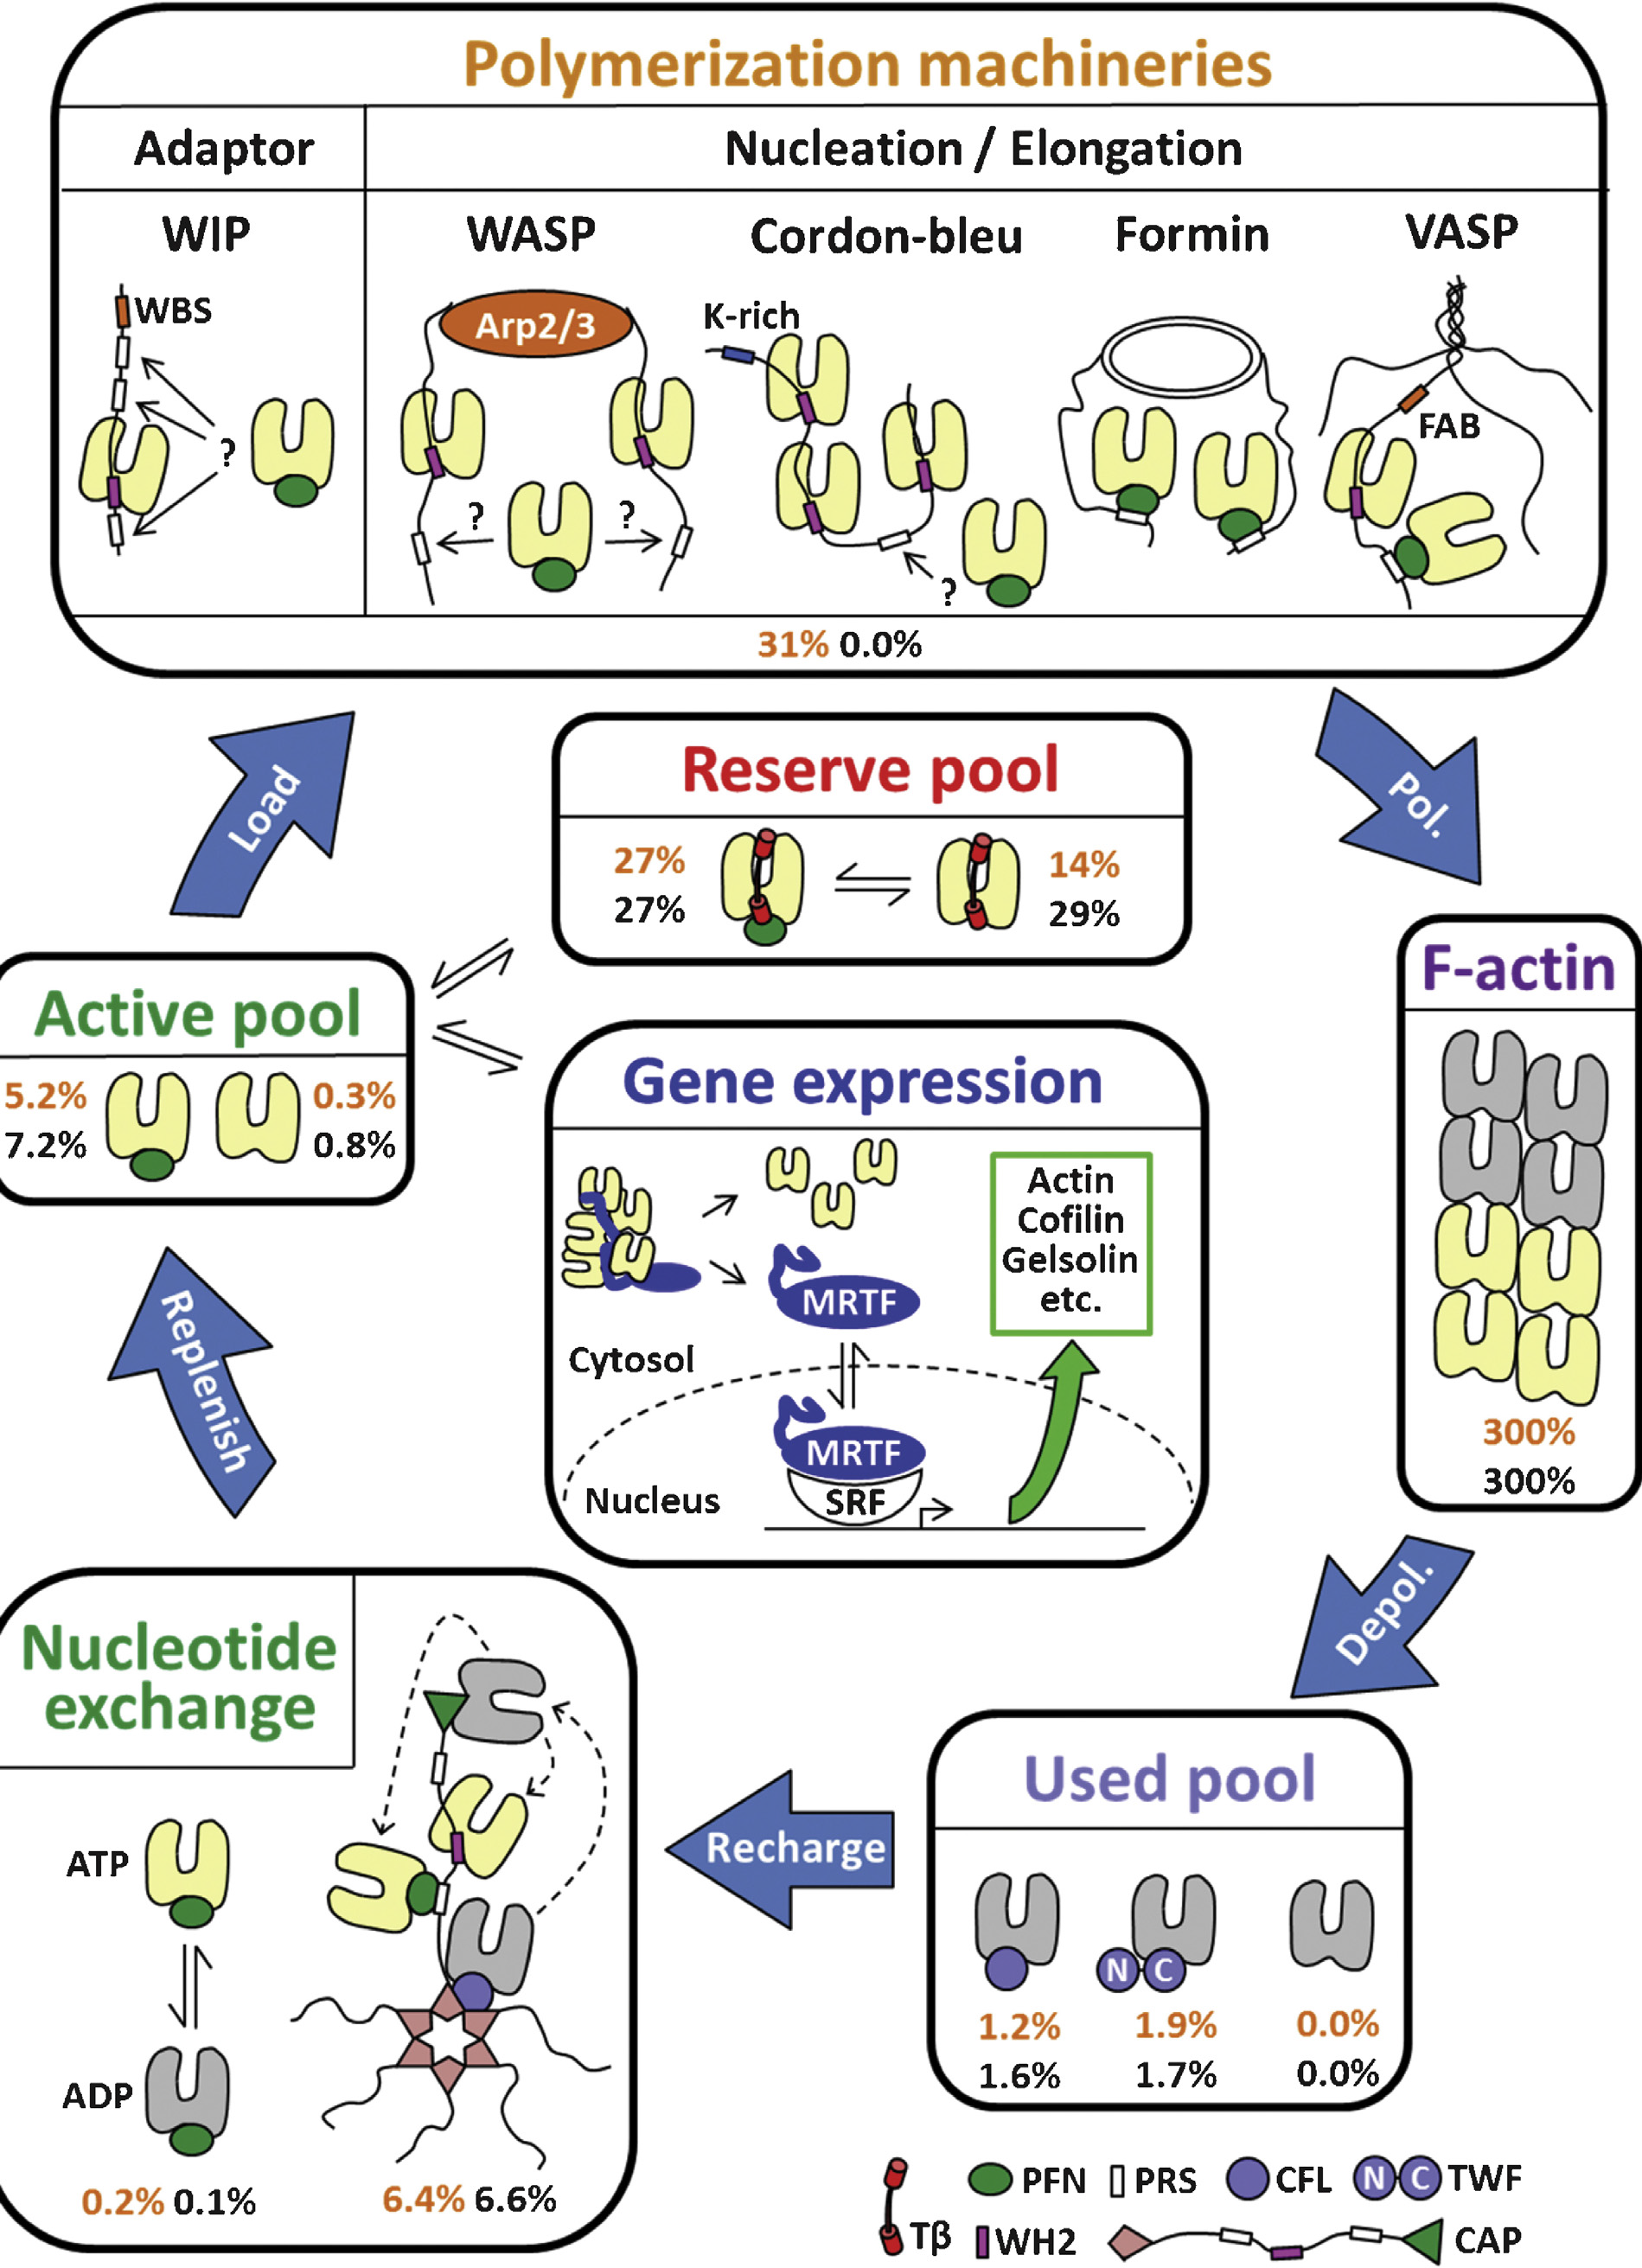
\includegraphics[scale=0.25]{actine_cycle.png}
\caption{Cycle de polymérisation et dépolymérisation de l'actine dans la cellule sous l'effet des différentes protéines liées à l'actine, d'après la revue de \cite{xue}. PFN : profiline, PRS : proline rich sequence, CFL : cofiline, TWF : twinfiline, WH2 : Wiskott-Aldrich syndrome homology region 2, T$\beta$ : thymosine $\beta$. } 
\end{figure}

\section{Actine F}

La principale fonction de l'actine chez les eucaryotes est sa capacité à former un réseau de filaments branchés, connecté par des moteurs moléculaires. 
La formation de filaments d'actine est régulée par de très nombreuses protéines qui vont se lier aux monomères ou aux filaments. 

\begin{figure}
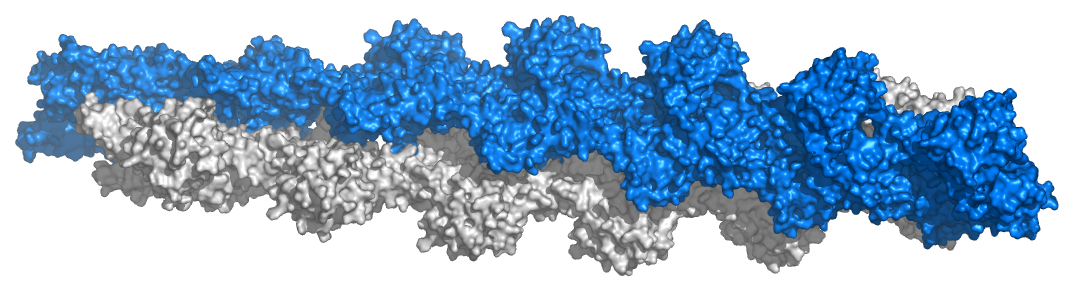
\includegraphics[scale=0.3]{Actin_filament_atomic_model.png}
\caption{Structure d'un filament d'actine basée sur le modèle de Ken Holmes, illustré par Thomas Splettstoesser}
\end{figure}

\subsection{Le filament}

Les filaments d'actine sont très dynamiques, et ont une structure changeante. Ils ont un diamètre de 6nm et une longueur de persistance de l'ordre de la dizaine de microns, donc du même ordre de grandeur que la taille typique cellulaire. 

Les monomères d'actine s'associent les unes à la suite des autres, l'extrémité pointue d'un monomère se liant à l'extrémité barbée de l'autre, avec une rotation entre un monomère et l'autre. 
Le filament est alors polarisé, avec une extrémité pointue notée également - et une extrémité barbée notée +. 

L'actine ATP est plus facilement polymérisée alors que l'actine ADP est plus facilement dépolymérisée. 
Les actines ATP incorporés dans un filament sont ensuite hydrolysées, et deviennent donc plus facilement dépolymérisables.
Les deux bouts du filaments ont alors des affinités différentes pour les monomères. En présence d'une grande quantité de monomères disponibles, le filament peut croître par les deux bouts, mais dans une concentration intermédiaire, le filament va croître par ajout de monomères à son extrémité + et décroître par dépolymérisation à l'extrémité -. L'équilibre entre les deux cinétiques de réaction détermine si la taille du filament croît ou non. 

Cet équilibre est connu comme le \og tapis roulant \fg de l'actine : lorsque les deux cinétiques sont égales, le filament avance par remplacement des monomères en gardant une longueur constante. 

Bien que cet assemblage puisse avoir lieu spontanément en présence d'actine, de nombreuses protéines aident à la nucléation des filaments, à leur stabilité ou à leur déstabilisation. 

\subsection{L'équilibre de polymérisation}

Des protéines vont réguler toute l'existence d'un filament d'actine : la nucléation, la croissance, la stabilisation et la dissociation. 

\subsubsection{Les nucléateurs}
Les dimères et les trimères d'actine sont des structures peu stables, à la durée de vie assez courte. C'est à partir du tétramère que la structure devient suffisamment stable pour créer un nouveau filament d'actine. 

Afin de dépasser cette barrière, d'autres protéines jouent le rôle de nucléateurs. Le complexe Arp2/3 (Arp pour Actin Related Protein) est le plus connu de ces nucléateurs. Il se lie au côté d'un filament et Arp2 et Arp3 miment un dimère d'actine. D'autres monomères peuvent alors se fixer sur cette base et un nouveau filament peut croître. Ce nouveau filament est de plus attaché avec un angle d'environ 70 \degres au filament initial, créant un réseau branché (\cite{blanchoin}). 

Les formines se fixent à l'extrémité barbée d'un filament et y ajoutent successivement des monomères d'actine. Les formines peuvent nucléer un nouveau filament en stabilisant un dimère et en y ajoutant d'autres monomères. \cite{pring}. 

\subsubsection{Les élongateurs}

Une fois les filaments formés, des facteurs d'élongation comme les formines ou Ena/VASP, peuvent ajouter des monomères liés à la profiline à l'extrémité barbée du filament. 
Certaines formines avancent le long du filament tout en le construisant à partir de complexes actine-profiline \cite{otomo}. 


\subsubsection{Protéines de coiffage (capping proteins)}

Il existe deux sortes de protéines de coiffage : celles qui se lient à l'extrémité barbée et contribuent donc à réduire la polymérisation (comme CapZ, la gelsolin ou la tensine), et celles qui se lient à l'extrémité pointue, empêchant la dépolymérisation (comme la tropomoduline). 


\subsubsection{Protéines de fragmentation (severing proteins)}
Les protéines de fragmentation découpent et dépolymérisent les filaments d'actine. 

La cofiline se lie aux filaments d'actine ADP et entraîne une configuration où la rotation des monomères les uns par rapport aux autres est plus grande \cite{mcgough}. Cela déstabilise les filaments et les casse. 

La gelsoline, la famille des villines et la fragmine sont également des facteurs de dépolymérisation des filaments d'actine. 

À première vue, on peut voir l'impression que ces protéines vont avoir tendance à diminuer le nombre et la longueur des filaments et participer à la destruction du cytosquelette. Cela peut être le cas, mais pas toujours : la fragmentation d'un long filament en de nombreux filaments courts fait apparaître de nombreuses extrémité barbées là où il n'y en avait qu'une seule. Selon les conditions, en particulier l'activation de facteurs d'élongation et la disponibilité des monomères, la fragmentation peut donc agir en faveur de la polymérisation, en particulier lors du remplacement d'un réseau à longs filaments par un réseau très dense et réticulé. 

Les protéines MICAL forment une famille de protéines dépolymérisant l'actine, découvertes récemment dans les neurones (\cite{hung_direct_2011}. En oxydant l'actine des filaments, elle les dépolymérise. Comme l'actine oxydée ne peut plus former de nouveaux filaments, la destruction du cytosquelette par MICAL ne peut pas promouvoir la croissance du réseau. 

MICAL2 est un membre de la famille des protéines MICAL qui est particulièrement localisé dans le noyau. L'actine qu'elle oxyde, en plus d'être dépolymérisée, est expulsée du noyau et ne peut plus y entrer (\cite{lundquist_redox_2014}). MICAL2 organise donc la régulation de l'actine nucléaire en appauvrissant le réservoir d'actine nucléaire en filaments et en monomères.

\subsubsection{Stabilisateurs des filaments}

Les tropomyosines sont des protéines qui vont former également des filaments. Ces filaments vont s'enrouler autour des filaments d'actines et les protéger : ils bloquent l'activité des cofilines et avec la troponine ils régulent l'association avec les myosines, en particulier dans la contraction musculaire (voir le chapitre 4).

\begin{figure}
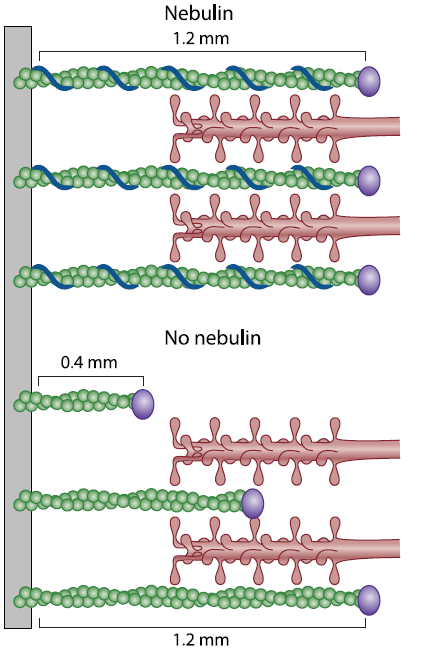
\includegraphics[scale=0.5]{Figures/Nebuline.png} 
\caption{Rôle de la nébuline dans le maintient de la longueur des filaments adéquate dans les cellules musculaires, d'après \cite{Ottenheijm}.\label{nebuline}}
\end{figure} 

Les nébulines sont des protéines stabilisantes dont le but est de fixer la longueur du filament d'actine auquel elles vont se lier, à la manière d'un étalon de mesure (\cite{Ottenheijm}, voir figure \ref{nebuline}). 



\subsection{Organisation en réseau de filaments}

Les filaments d'actine en évolution permanente sont liés entre eux mais également à la membrane plasmique et aux autres filaments du cytosquelette (microtubules et filaments intermédiaires). 


\subsubsection{Ancrage à la membrane}

Les cellules sont liées mécaniquement entre elles par les cadhérines qui relient leur réseau d'actine. Les caténines font la liaison entre les cadhérines et les filaments d'actine. 

L'ancrage du cytosquelette à la matrice extra-cellulaire se fait par l'intermédiaire d'une structure extraordinairement complexe, les adhésions focales. 
Au niveau des adhésions focales, des dizaines de protéines interagissent entre elles pour relier les intégrines enchâssées dans la membrane et les filaments d'actine. 
Je ne vais pas faire ici l'inventaire des protéines impliquées dans ces adhésions. 
À l'intérieur des adhésions focales, une signalisation complexe est à l'\oe uvre qui permet, en réponse à des forces extérieures, de construire une structure mécanosensible capable de déclencher des cascades de signalisation dans toute la cellule \cite{geiger}. 
En particulier, les petites GTPases Rac, Rho et Ras sont activées par des signaux provenant des adhésions focales soumises à des signaux mécaniques et régulent l'architecture du cytosquelette.
Je reviendrai plus loin sur la mécanique des adhésions focales.  

\subsubsection{Protéines de pontage}

Les filaments d'actine sont organisés en réseau par des protéines comme la filamine, la spectrine ou la transgeline. 

\begin{figure}
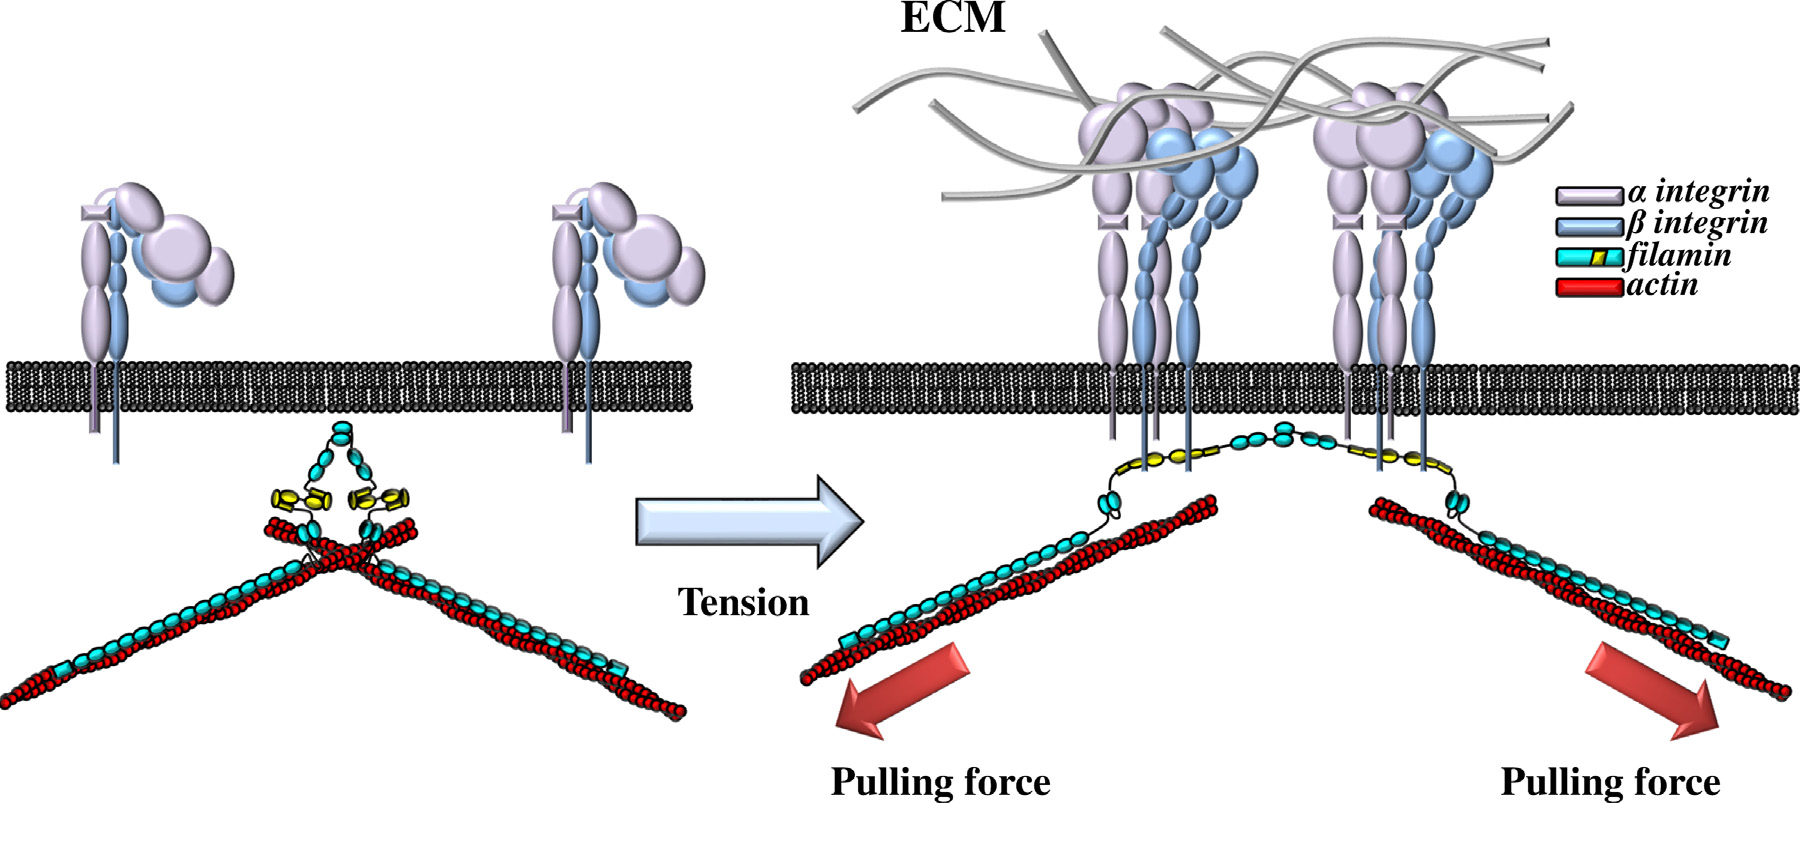
\includegraphics[scale=0.25]{Figures/filamine.png} 
\caption{Représentation d'un dimère de filamine se dépliant sous tension par \cite{janostiak} \label{filamine}}
\end{figure}

La filamine est un homodimère qui lie deux filaments d'actine. Elle peut se déformer sous la contrainte \cite{furuike}, ce qui permet de doter le réseau d'actine à la fois d'une élasticité et d'une mécanosensibilité supplémentaire \cite{kainulainen}.
La filamine peut également se lier à la membrane pour y ancrer le réseau d'actine  \cite{yamazaki}.


Lorsque son interaction avec les filaments est forte, l'$\alpha$-actinine peut lier des filaments en réseaux, alors que lorsque sa vitesse de dissociation est grande elle forme plutôt des faisceaux \cite{Wachsstock}. Elle fait partie des protéines qui organisent les filaments d'actine dans les cellules musculaires, et sera donc évoquée à nouveau dans le chapitre 4. 


\subsubsection{Protéines de faisceau}

Ces protéines permettent de rassembler les filaments d'actine en faisceaux parallèles ou anti-parallèles. Cette architecture est retrouvée dans les filopodes, dans les fibres de stress ou dans les microvillosités.

Il peut y avoir deux domaines de liaison à l'actine sur la même protéine, comme c'est le cas pour la fimbrine, l'écart entre deux filaments est alors faible et le faisceau maintenu serré. 
Des protéines se liant à l'actine peuvent également former des dimères ou des multimères où chaque sous-unité lie un filament. L'$\alpha$-actinine permet ainsi de former des fibres de filaments anti-parallèles. La jonction entre les filaments est plus souple et moins serrée. 

\subsubsection{Lien avec les autres filaments du cytosquelette}

Le cytosquelette d'actine est relié aux réseaux de filaments intermédiaires et aux microtubules par des protéines capables de se lier à deux ou aux trois types de filaments. 
Par exemple, la plectine et les nesprines permettent de connecter les microtubules et les filaments d'actine au réseau de lamines de la membrane nucléaire, et donc de transmettre les contraintes jusqu'au noyau. 
Les WHAMM en sont un autre exemple, elles se lient aux microtubules et à la membrane et nucléent des filaments d'actine. 


 



\subsubsection{Moteurs moléculaires : myosines}

Les myosines sont des moteurs moléculaires qui se déplacent sur l'actine en consommant de l'ATP. Il en existe chez tous les eucaryotes, mais leur homologie n'est pas aussi grande que celle de l'actine, car elles ont des fonctions différentes. Dans le génome humain, on dénombre une quarantaine de gènes pour la myosine, qui forment 17 groupes.

\begin{figure}
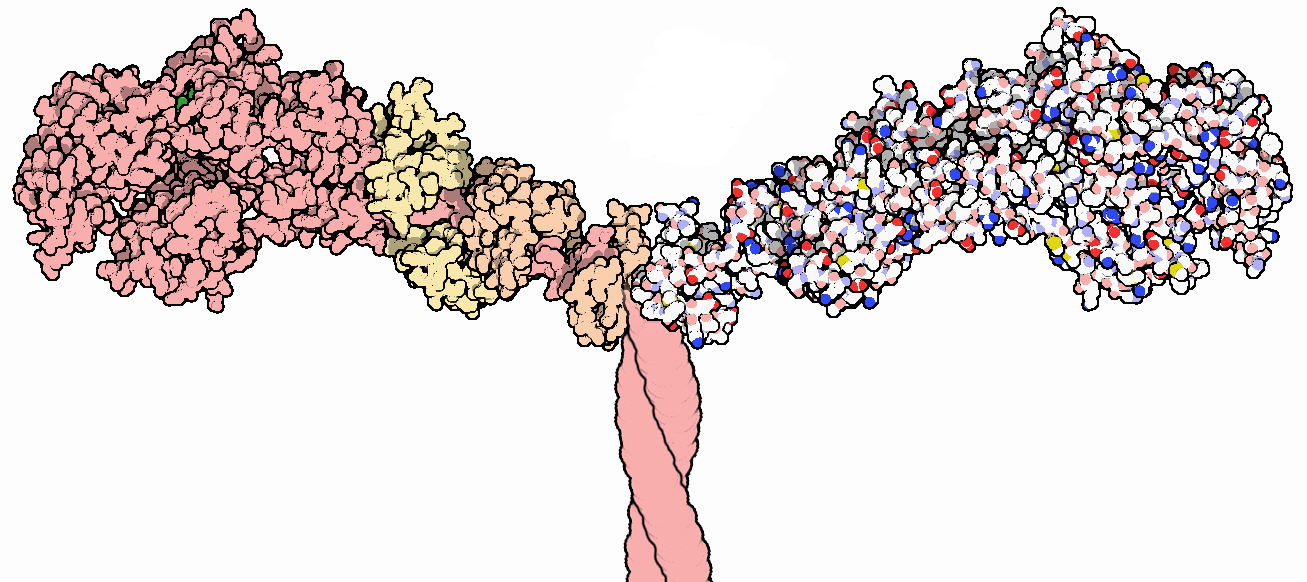
\includegraphics[scale=3]{Figures/18-Myosin-1b7t.png} 
\caption{Structure d'une myosine à deux têtes : en rouge la chaîne lourde, en jaune et orange les deux chaînes légères. Les queues des deux chaînes lourdes sont enroulées l'une autour de l'autre. Illustration tirée de l'article du mois de la Protein Data Bank sur la myosine \cite{goodsell} \label{myosin}}
\end{figure}

La myosine II, aussi appelée \og conventionnelle \fg est la plus étudiée. Elle est présente en quantité importante dans le muscle, car avec l'actine elle permet la contraction musculaire. 

Les myosines ont une tête qui peut se lier à l'actine en filament, un cou  qui sert de levier et de régulateur, et une queue qui sert souvent à former un dimère, et éventuellement à se lier à un cargo. On les appelle "chaînes lourdes" par opposition aux \og chaînes légères \fg, qui ne sont pas à proprement parler des myosines mais qui sont des protéines qui vont se lier au cou des \og chaînes lourdes \fg pour les réguler. On peut en voir une représentation par la Protein Data Bank en figure \ref{myosin}.

Par exemple, pour la contraction musculaire, deux chaînes lourdes de myosine II s'associent en dimère par leur queue, et quatre chaînes légères s'ajoutent au niveau des deux cous. Les queues de milliers de myosines sont tressées en un filament épais, qui va coulisser par rapport au filament d'actine, appelé en comparaison filament fin, sous l'action du cycle de la myosine (voir figure \ref{myosin_cycle}. La structure et la contraction musculaires seront détaillées dans le chapitre 4. 

Le dimère a alors deux têtes pouvant se lier à l'actine, et va s'en servir pour avancer le long du filament, à la manière dont un alpiniste plante un piolet, se hisse puis détache le piolet pour le replanter plus loin, successivement pour les deux bras. Le cycle de la myosine est présentée en figure \ref{myosin_cycle}. 

\begin{figure}
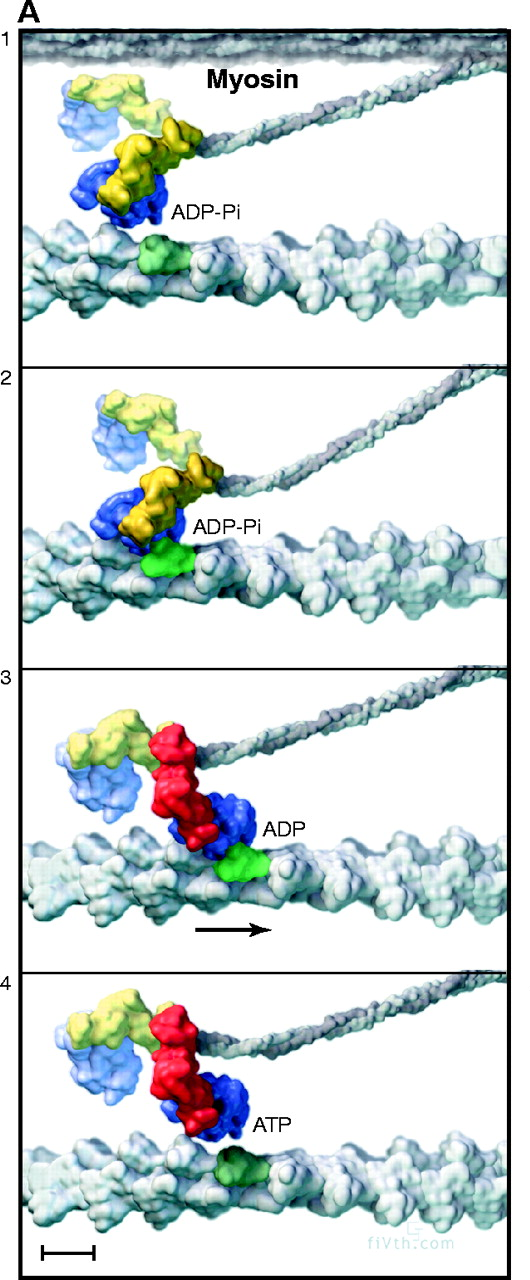
\includegraphics[scale=0.5]{Figures/Myosin.png} 
\caption{Reconstitution du cycle de la myosine à l'aide des données de la Protein Data Bank par \cite{Vale}. Ici deux myosines forment un dimère doté de deux têtes et d'une longue queue qui lui permet de se lier au filament épais, composé de milliers de queues de myosines.  1 $\rightarrow$ 2 : La tête de myosine liée à un ADP + phosphate se lie au filament d'actine. 2 $\rightarrow$ 3 : Le phosphate est libéré, causant un changement de conformation du levier (en jaune sur l'image 2, en rouge sur l'image 3) qui fait coulisser un filament par rapport à l'autre. 3 $\rightarrow$ 4 : L'ADP est remplacé par un ATP, ce qui provoque le détachement du filament d'actine. 4 $\rightarrow$ 1 : L'ATP est hydrolysé en ADP+Pi, ce qui arme la tête de myosine, préparant le cycle suivant. La barre représente 6nm. \label{myosin_cycle}}
\end{figure} 





Certaines myosines ont un rôle analogue à celui des moteurs moléculaires associés aux microtubules et transportent des molécules le long des filaments, en général en direction de l'extrémité + ,seule la myosine VI se déplace en sens inverse. Certaines autres, comme les myosines I n'ont qu'une seule tête. 


Les faiceaux anti-parallèles d'actine peuvent être liés par des paires de dimères de myosine, qui vont marcher en sens opposé sur les deux filaments, et donc les déplacer l'un par rapport à l'autre. Si les deux filaments sont liés par ailleurs dans le réseau, il va être mis sous tension par ces moteurs moléculaires. 




\section{Rôle mécanique de l'actine : du filament au cytosquelette}

Le cytosquelette est une structure multi-échelle, allant de l'échelle des protéines, à l'échelle de la cellule toute entière, en passant pas l'échelle des filaments et des réseaux de filaments. Il peut ressentir et exercer des forces à toutes les échelles. 


Dans cette partie, il ne s'agit pas de parler des propriétés mécaniques du cytosol ou de la cellule, mais d'expliquer comment les filaments peuvent générer des forces et comment ils réagissent à des forces. 

\subsection{Mécanique du filament d'actine}

Le filament d'actine en lui-même est à la fois générateur et senseur de forces. 

 \subsubsection{Longueur de persistance}
La longueur de persistance est un moyen de quantifier la corrélation entre l'orientation des différents segments d'un polymère soumis aux fluctuations thermiques. Si l'on considère un polymère de longueur $L$ auquel on attribue une abscisse curviligne $s$, avec $\vec{t_s}$ la tangente au polymère en $s$, alors on a la relation : 
$$ \langle \vec{t_0}\cdot \vec{t_s} \rangle_L \propto e^{-L/\ell_p}$$

Au bout de quelques longueurs de persistance, l'information de l'orientation du polymère en $s=0$ est perdue. 

La longueur de persistance dépend de l'énergie thermique disponible pour agiter le filament : elle diminue lorsque la température augmente. 

On peut également définir l'énergie de courbure d'un filament de longueur $L$, de rayon $a$ et de module d'Young $E$ : 
$$ E= \frac{\kappa}{2L} \int_0^L \left( \frac{\partial \theta}{\partial s} \right) ds \approx \frac{\kappa L}{2R^2}$$
 où $\kappa \approx Ea^4$ est le module de courbure et $R$ le rayon de courbure du filament.  
 On définit alors la longueur de persistance comme la longueur pour laquelle l'énergie de courbure devient comparable à l'énergie thermique : 
 $$ E (L=l_p,R=l_p) = \frac{k_B T}{2} = \frac{\kappa l_p}{2 l_p^2}$$ 
 $$ l_p = \frac{\kappa}{k_B T}$$
 
 


Le filament d'actine subit un vieillissement par l'hydrolyse de l'ATP des monomères qui le composent. Le changement de conformation induit par l'hydrolyse de l'actine a des conséquences sur les propriétés mécaniques du filament. 
Un filament d'actine ATP a une longueur de persistance de 15 micromètres, contre 9 micromètres pour un filament d'actine ADP \cite{isambert}. Le vieillissement du filament le rend donc plus déformable et plus souple. 
Les protéines attachées au filament peuvent également, en stabilisant une conformation, changer sa rigidité. Un filament stabilisé par la phalloïdine ou par la tropomyosine voit sa longueur de persistance augmentée à 18 et 20 microns respectivement \cite{isambert}. Au contraire, la conformation stabilisée par la cofiline n'a qu'une longueur de persistance de 2,2 microns \cite{mccullouch}. 

Un même filament d'actine peut évidemment être le lieu de toutes ces modifications en même temps. Souvent l'extrêmité + des filaments est riche en actine ATP alors que l'extrémité - est riche en actine ADP, ce qui crée un filament plus rigide d'un côté et plus flexible de l'autre. 

\subsubsection{Couplage traction-torsion}

L'hélice que forme le filament peut adopter des conformations différentes, en particulier en ce qui concerne l'angle de rotation entre les monomères successifs. 
Une force tirant sur le filament va alors favoriser une conformation à faible torsion, ce qui va rendre la fixation de la cofiline, qui stabilise le filament dans une conformation à grande rotation, beaucoup plus difficile. 
Il en résulte que la cofiline est moins efficace sur les filaments qui sont en tension \cite{hayakawa}, induisant une préservation automatique des filaments sous contrainte par rapport aux filaments libres. 
Au contraire, la formine mDia1, qui est un élongateur des filaments, et la profiline sont plus efficaces sur les filaments soumis à une tension \cite{higashida}. 
La conformation de l'actine est alors un senseur de contrainte qui va encourager la préservation et l'élongation des filaments qui ressentent une force de traction. 

Les filaments d'actine semi-flexibles peuvent également être courbés, en particulier au voisinage de la membrane. 
À cause de l'organisation hélicoïdale des monomères, la courbure d'un filament d'actine exerce également une torsion sur ce filament, ce qui rend la modélisation des filaments encore plus complexe. 
Des observations \textit{in vitro} sur des filaments d'actine courbés et immobilisés montrent que le facteur de nucléation Arp2/3 se lie préférentiellement au côté convexe d'un filament d'actine courbé \cite{risca}. 

\subsubsection{Les myosines}

Le cycle de la myosine, voir \ref{myosin_cycle} est lui-même dépendant des contraintes qui peuvent être appliqués à la myosine. 
L'application d'une force de 1,6pN poussant la myosine vers sa conformation finale divise par deux la durée que la myosine va passer attachée au filament en facilitant le changement de conformation \cite{veigel}. 
Inversement, l'application de la même force en sens opposé multiplie par deux la durée d'attachement. 
En fait, la durée que la myosine passe attachée au filament d'actine dépend exponentiellement de la force exercée, dans la gamme -2pN $-$ 2pN \cite{veigel}. 

Les forces transmises par les filaments sous tension vont donc influer sur la cinétique du cycle de la myosine, et donc sur les forces qui vont être exercée par elle sur les filaments. 

\subsubsection{La croissance du filament comme source de force}

La croissance des filaments peut elle-même être une source de forces. Par exemple, un filament en croissance proche de la membrane plasmique s'appuie sur elle et sur le réseau d'actine derrière lui dans la cellule. La bactérie \textit{Listeria Monocytogenes} utilise ce mécanisme pour se déplacer à l'intérieur des cellules qu'elle infecte : elle possède à une extrémité des protéines Arp2/3 qui polymérisent l'actine. 

Ces forces peuvent également être utilisées pour pousser la membrane plasmique, créant une protrusion comme un filopode ou un lamellipode. Sous l'effet de l'agitation thermique, un monomère pousse la membrane. Si l'extrémité barbée d'un filament se trouve à proximité, le monomère peut alors rejoindre le filament. Ce qui était une fluctuation thermique devient alors une déformation pérenne de la membrane plasmique par le filament d'actine. 

\begin{figure}[h!]
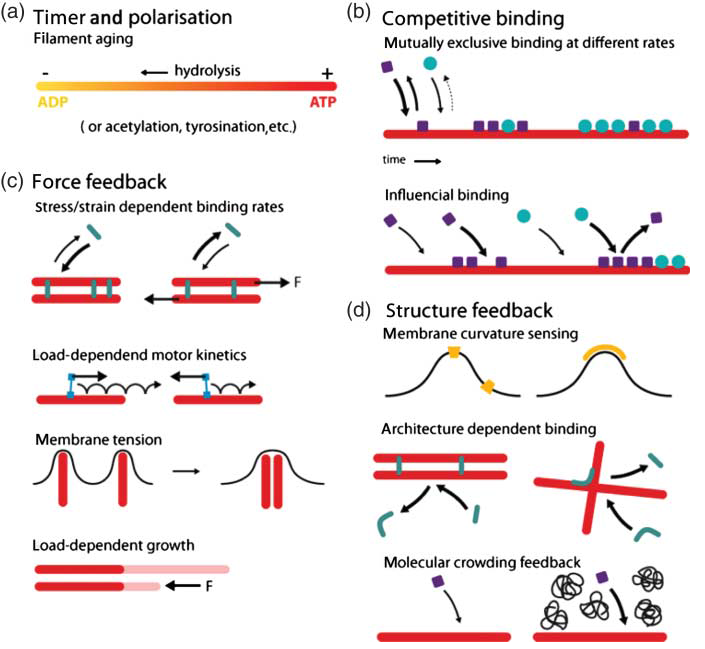
\includegraphics[scale=0.7]{Actine_phenomenon.png}
\caption{Présentation des différentes sources de sensibilité mécanique du cytosquelette d'actine au niveau du filament lui-même et des protéines interagissant avec lui, d'après la revue de \cite{huber}}
\end{figure}



\subsection{Mécanique des adhésions focales}

Les sites d'ancrage de la cellule dans la matrice extra-cellulaire sont la porte d'entrée des signaux mécaniques dans la cellule. Parmi les molécules qui constituent les adhésions focales, certaines réagissent directement lorsqu'elles sont soumises à des stimulations mécaniques. 

Lorsque la transmission des forces est coupée dans la cellule (par l'ajout de drogues qui inhibe la contractilité du cytosquelette), les adhésions focales disparaissent : la tension est nécessaire non seulement à leur constitution, mais également à leur maintien. Ces contraintes peuvent provenir de forces extérieures mais aussi de la contraction du cytosquelette sous l'action des moteurs moléculaires. 

\begin{figure}
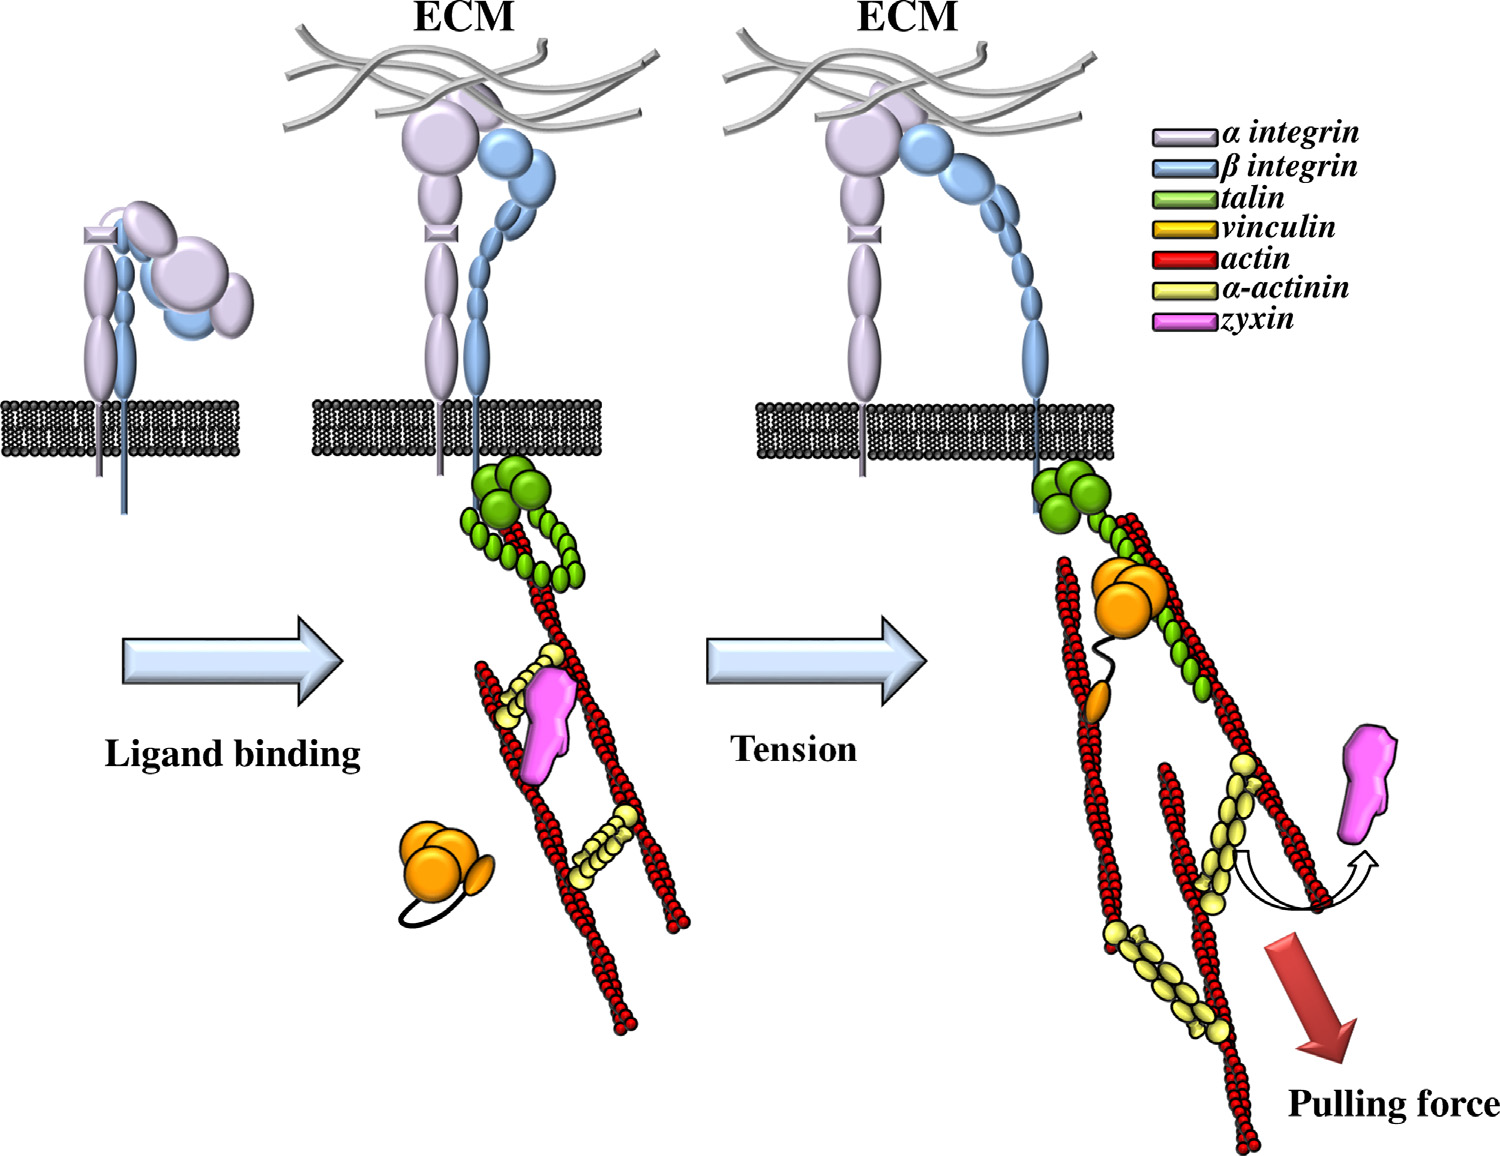
\includegraphics[scale=0.2]{Focal_adhesions_taline.png}
\caption{Dépliement de la taline sous tension, qui fait apparaître les sites cryptiques de liaison à la vinculine, d'après \cite{janostiak}}
\end{figure}

En présence d'une force, les intégrines forment des agrégats et leur affinité pour le ligand augmente grâce à un changement de conformation. 
La taline relie les intégrines aux filaments d'actine. Dans la conformation initiale, elle est repliée sur elle-même. Lorsqu'elle est mise sous tension entre les intégrines et l'actine, elle se déplie, laissant apparaître des domaines de liaisons à la vinculine qui n'étaient pas précédemment accessibles \cite{delrio}. 
L'arrivée des vinculines dans les adhésions focales dépend de la tension au niveau de l'adhésion \cite{pasapera} et permet leur renforcement \cite{galbraith}. 

La filamine, qui lie entre eux des filaments d'actine, peut être dépliée lors de tensions sur les filaments  \cite{furuike}. Son domaine de liaison aux intégrines devient alors accessible, et la filamine ancre alors le cytosquelette à la matrice extra-cellulaire par l'intermédiaire des intégrines \cite{yamazaki}. De plus, cela cause un changement de conformation des intégrines qui favorise la formation d'agrégats, renforçant l'adhésion. Cela est illustré par la figure \ref{filamine}.

Ce ne sont là que quelques exemples de protéines impliquées dans les adhésions focales, il en existe des centaines. Leur exemple montre qu'au premier niveau de contact avec l'environnement mécanique extérieur, les forces sont relayées en un signal biologique au niveau de la molécule individuelle, en changeant la conformation des protéines. 

\subsection{Mécanique du cytosquelette d'actine}

Les protéines organisant les filaments d'actine vont construire des structures à l'échelle de la cellule spécialisées dans l'exploration, le mouvement, le maintien ou le changement de forme \dots

Le cytosquelette  a principalement été étudié par la motilité sur des surfaces planes et rigides de cellules comme les fibroblastes et les kératocytes. 
Cependant, d'autres types cellulaires peuvent s'engager dans des mouvements ou des organisations du cytosquelettes très différentes. 
C'est le cas par exemple des cellules du système immunitaire : par exemple les lymphocytes T patrouillant dans le système sanguin sont dotés d'un uropode qui leur permet de s'orienter à contre-courant \cite{valignat}. Autre exemple, la phagocytose requiert une réorganisation polarisée rapide du cytosquelette à l'échelle de la cellules.
C'est également le cas des cellules musculaires différenciées en myofibres, qui ont une organisation du cytosquelette extrêmement spécialisée pour la contraction musculaire, et qui seront décrites plus loin au chapitre 4. 

Si les organisations décrites ici ont été particulièrement étudiées dans le cadre des fibroblastes et des kératocytes, elles font partie des mécanismes de migration de la plupart des cellules. 

\subsubsection{Le cortex}

La membrane plasmique est soutenue par un réseau d'actine de quelques centaines de nanomètres d'épaisseur appelé le cortex.

Le cortex est constitué d'un mélange entre un réseau ramifié par Arp2/3 et des faisceaux de filaments alignés. 
Il est attaché à la membrane plasmique par des protéines comme celles de la famille ERM (ezrine, radixine, moesine). 

Il contient également des myosines qui mettent le réseau sous tension. Cette tension crée une pression vers l'intérieur de la cellule contrée par la pression osmotique. 
Lorsque le cortex d'actine est brisé ou détaché de la membrane localement, cette pression interne de la cellule provoque la formation d'une protrusion de la cellule appelée bleb. 

Les blebs sont un moyen qu'a la cellule d'explorer l'espace. La protrusion de membrane est alors complétée par un réseau d'actine et des adhésions à partir desquels la cellule va pouvoir se tracter vers l'avant. 
Ce mode de déplacement a été particulièrement étudié chez les amibes comme Dictyostelium, c'est pourquoi il est dit \og amiboïde \fg.  

Le cortex et la membrane sont intimement couplés mécaniquement, au point qu'il est souvent difficile de séparer l'influence mécanique de la tension de la membrane de celle du cortex. 
En aspirant le cortex dans une micropipette il est possible de tester la résistance mécanique du cortex, et de constater qu'elle dépend de l'activité des myosines. 



\subsubsection{Le lamellipode}

Le lamellipode est une structure plane à l'avant d'une cellule en mouvement, prenant la plupart du temps une forme en croissant. 

Sous la membrane, la GTPase Rac active Arp2/3 par l'intermédiaire du complexe WAVE, formant un réseau ramifié.
La croissance des filaments pousse alors le bord de la cellule vers l'avant, en s'appuyant sur les adhésions focales à l'arrière du lamellipode. 
La croissance du réseau ramifié créé par Arp2/3 est maintenu sous contrôle par les protéines de coiffage qui bloquent l'élongation excessive des filaments. 

Le flux rétrograde de l'actine entraîne les filaments vers l'arrière de la cellule où ils sont fragmentés et dépolymérisés. 
Certains sont assemblés en faisceaux contractiles par les myosines. 

À l'arrière de la cellue, le réseau d'actine est détruit et les adhésions disparaissent afin de permettre à la cellule d'avancer. 

Le lamellipode est principalement lié aux déplacements sur une surface plane, comme en culture cellulaire ou à la surface d'un épithélium. 


\subsubsection{Les filopodes}

Les filopodes sont des protrusions consituées d'un faisceau d'actine dont les extrémité $+$ sont pointées vers l'extérieur. 
La croissance du filopode est principalement liée à celle des filaments du faisceau grâce à l'action des formines ou de Ena/VASP. 

Un filopode peut se former à partir de la convergence de filaments provenant d'un réseau branché au bord de la cellule. 
Des protéines comme la fascine associent alors ces filaments en faisceau rigide, dont la croissance déforme la membrane plasmique. 

Les filopodes servent à explorer l'espace, initiant le contact avec la matrice extra-cellulaire ou avec d'autres cellules voisines. 
Certaines bactéries exploitent ce comportement pour être capturées et internalisées par la cellule. 
Après contact avec la bactérie, le filopode se rétracte rapidement, ramenant la bactérie vers sa cible.
La force exercée par un filopode en rétraction peut atteindre 10pN, à des vitesses de l'ordre de 100nm/s. 



\subsubsection{Fibres de stress}

Les fibres contractiles sont constituées de faisceaux de filaments anti-parallèles associées à des myosines. 
Les fibres de stress sont des structures qui apparaissent essentiellement dans les cellules étalées sur un substrat plan, beaucoup plus rarement dans une matrice à trois dimensions. 

\section{Rôle régulateur de l'actine nucléaire}

L'actine nucléaire est plus difficile à observer que l'actine cytoplasmique, c'est pourquoi son existence et son rôle ont été ignorés pendant longtemps. 
Aujourd'hui, l'amélioration des techniques de microscopie et le développement de techniques spécifiques (comme des sondes dotées d'un NLS) permettent de confirmer l'existence d'actine nucléaire tant en monomères qu'en filaments (\cite{mcdonald_nucleoplasmic_2006},\cite{baarlink_nuclear_2013}). 
De plus, un grand nombre de protéines liées à l'actine, comme la profiline, la cofiline, Arp2/3, N-WASP, les formines, MICAL et des myosines, sont également présentes dans le noyau, créant toutes les conditions pour qu'un véritable nucléosquelette soit constitué dans la cellule. 
La profiline et la cofiline aident respectivement à l'export et à l'import des monomères d'actine par les pores nucléaires, jouant ainsi un double rôle de régulation de l'actine nucléaire. 


\subsection{L'actine G nucléaire dans les complexes}

80\% de l'actine nucléaire est sous forme de monomères. Ces monomères vont s'incorporer dans un grand nombre de complexes indispensables à la transcription de l'ADN en ARN et à la maturation de l'ARN. 

Chez les eucaryotes, la transcription de l'ADN en ARN est effectuée par trois ARN Polymérases. Il a été montré que l'actine est nécessaire à l'activité des trois ARN Polymérases ( \cite{Ye} \cite{Hoffman} \cite{Hu}).

L'actine est également liée aux ribonucléoprotéines hétérogènes (hnRNP) présentes sur les pré-ARN messagers pendant et après leur transcription \cite{kukalev}. Les hnRNP empêchent ces ARN messagers qui doivent encore subir des étapes de maturation de se replier sur eux-mêmes (ce qui pourrait interférer avec leur traitement) ou d'être exportés avant d'avoir été traités. Elles peuvent également se lier à la machinerie d'épissage. 

Les complexes de remodelage de la chromatine font passer la chromatine d'un état très compact impossible à transcrire à un état où l'expression des gènes devient possible. L'actine fait partie de plusieurs types de complexes de remodelage de la chromatine comme SWI/SNF, RSC et BAF (revue par \cite{Farrants}. 

Enfin, l'actine monomérique bloque également l'activité de la DNase I dans le noyau et l'empêche de couper l'ADN en petits morceaux \cite{lazarides}. 

\subsection{Les filaments d'actine et la myosine nucléaires}

20\% de l'actine nucléaire est présente sous la forme de filaments \cite{mcdonald_nucleoplasmic_2006}. Les nucléateurs comme Arp2/3 \cite{Yoo} et les formines \cite{baarlink_nuclear_2013} sont présents dans le noyau, aux côtés d'élongateurs spécifiques comme l'émerine \cite{ho_lamin_2013}. 
Des myosines, comme la Nuclear Myosin 1 (NM1) \cite{nowak}  et la myosine VI sont présentes dans le noyau et ont un rôle essentiel dans la transcription. 

L'actine, mais également N-WASP et Arp2/3 sont nécessaires à la transcription efficace par l'ARN Polymérase II \cite{Yoo}. Les drogues empêchant la formation de filaments comme la latrunculine ou la cytochalasine D perturbent la transcription par PolII \cite{mcdonald_nucleoplasmic_2006}.

La NM1 et l'actine se lient à PolI pour la transcription des gènes ribosomaux. La NM1 remodèle localement la chromatine dans une conformation favorable à la transcription \cite{nowak}.

L'émerine, qui relie des filaments d'actine aux lamines qui enveloppent le noyau, joue un rôle essentiel dans l'organisation de l'hétérochromatine (revue par\cite{gieni}). 


Le noyau contient tous les éléments nécessaires à la formation d'un nucléosquelette mécaniquement fonctionnel : nucléateurs, élongateurs, protéines de pontages et moteurs moléculaires. 
Ce nucléosquelette est relié au cytosquelette par différentes protéines de la membrane nucléaire qui lient l'actine F, les filaments intermédiaires, les microtubules et les centrosomes. 
Dans le cas de l'actine, les nesprines et Sun 1 et 2 font la liaison entre les filaments d'actine du cytoplasme et les lamines, qui font la liaison avec les filaments nucléaires et la chromatine grâce à l'émerine. 





\end{document}